\chapter{Introduction}
\label{chapter:intro}

%Introduction tells the motivation, scope, goal and the outcome of the
%work. Anyone should be able to understand it. The preferred order of
%writing your master's thesis is about the same as the outline of the
%thesis: you first discover your problem and write about that, then you
%find out what methods you should use and write about that.  Then you
%do your implementation, and document that, and so on.  However, the
%abstract and introduction are often easiest to write last.  This is
%because these really cover the entire thesis, and there is no way you
%could know what to put in your abstract before you have actually done
%your implementation and evaluation. This means that you have to
%rewrite them in the end of your work.

%By the way, rarely anyone write the thesis from the beginning to the
%end just one time, but the writing is more like process, where every
%piece of text is written at least twice. Be also prepared to delete
%your own text. In the first phase, you can hide it into comments that
%are started with \% but during the writing, the many comments should
%be visible for your helpers, the advisor(s) and supervisor.

%Read the information from the university master's thesis
%pages~\cite{ThesisInstructions} before starting the thesis.  You
%should also go through the thesis grading
%instructions~\cite{ThesisGrading} together with your advisor and/or
%supervisor in the beginning of your work.

%The introduction in itself is rarely very long; two to five pages
%often suffice. It usually has two subsections with titles Problem
%statement and Structure of the Thesis, as follows next.


\section{Problem statement}

Dense and accurate disparity maps are the key factor for obtaining correct depth estimations for many computer vision applications such as autonomous driving, 3D reconstruction, object detection and robotics.  
Therefore, stereo matching and disparity estimation can be identified as fundamental problems in the current developments of computer vision \citep{Seki2017}.\\
Multiple methods for disparity estimation has been developed for many years \citep{Seki2017}. 
Specifically, older strategies are focused on local-based or global-based methods. On the contrary, deep learning based strategies applied to local or global methods has been recently proposed. 
The latter approach aims to a precise local correspondence exploiting deep learning and applying Semi-global matching (SGM) as the regularization step of the pipeline. 
Therefore, deep learning techniques such as FlowNet and DispNet \citep{Seki2017} are used as the end-to-end part of the pipeline.
According to the current benchmark database ranks for stereo matching algorithms, e.g. the one published in the KITTI website, the state of the art implementations are based on deep learning methods. 
However, these strategies lack in accuracy compared to the standard pipelines. 
This is probably due to the difference between real environment and the training database as underlined in \citep{Seki2017} \citep{Poggi2019}.\\
As aforementioned, the state of the art methods to recover dense disparity maps from stereo pairs are focused on deep convolutional neural networks trained end-to-end \citep{Tonioni2020}. 
Most of these techniques, which will be subsequently described, exploit as regularization phase the Semi-global matching (SGM) method.
Actually, among local and global approaches, the Hirschmuller's algorithm \citep{Hirschmuller2008} appears to be the best performing in terms of computational cost and accuracy. 
For this reason, it is the preferred trade-off for most real time applications.\\
Considering the multiple algorithm for stereo correspondence, they can be conventionally classified \citep{Scharstein2001} into two general categories, local and global approaches.
Specifically, the local-based methods tend to estimate the disparity image trough a comparison of the matching cost from left and right views of the scene. 
In order to recover from low accuracy proper of the previous strategy, global-based methods try to calculate the disparity values by minimizing an energy function.
In this context, Semi-Global Matching (SGM) combines strong factors of global and local approaches allowing to obtain a good trade-off between computational cost and accuracy. \\
Technically speaking, SGM applies a pixelwise, Mutual Information (MI) based matching cost for analysing pixel intensity value differences of input images \citep{Hirschmuller2008}.
Moreover, pixelwise matching is enhanced with a smoothness constraint, which leads to a global cost function. 
Then, post-processing techniques are applied to remove outliers and filter the image.\\
Referring to the analysis performed by Scharstein and Szeliski \citep{Scharstein2001}, SGM carries out four main steps, as well as most of the stereo matching algorithms. 
These are defined as: matching cost computation, cost aggregation, disparity computation and disparity refinement. \\
Considering the former, it is usually based on absolute, squared or sampling insensitive difference between pixel intensities \citep{Hirschmuller2008}. Although those methods allow to reach a reliable accuracy, they are sensitive to radiometric difference. 
Thus, cost based on image gradients or window-based methods, such as rank and census transform \citep{Ko2017Ko2017}, became an optimal choice. 
Furthermore, Mutual Information results as a good trade-off for dealing with complex radiometric relationships between images.\\
In the second phase, cost aggregation collects the matching costs considering multiple directions and the disparity levels. 
Following, disparity evaluation is defined for each pixel, as the one with the lowest cost. This is the approach typically used for local methods. 
Global algorithms, rather, used to get rid of the aggregation step and define a global energy function. 
Over that function, pixel similarity and disparity smoothness are enforced with different strategies. In this latter case, the best disparity is identified finding the minimum of the cost function. This is achieved with multiple techniques such as: Dynamic Programming (DP) \citep{Birchfield1999}, Belief Propagation \citep{Klaus2006} or Graph Cuts \citep{Kolmogorov2001}.\\
Disparity refinement tends to differ more among the different methods. Usually, post-processing techniques such as filtering, outlier removal and consistency check are in general applied.\\
As anticipated above, among the top-ranked stereo matching algorithms, SGM results to be the best performing in terms of computational time and accuracy. 
Its benefits stand in the hierarchical computation of the matching cost, which exploit Mutual Information. 
Cost aggregation is achieved taking into account a global energy function and a pathwise pixel optimization. 
The final disparity is chosen with a winner takes all strategy. 
Disparity refinement is completed by consistency check between left and right disparity images. \\
Besides the challenge of building up the optimal algorithm for recovering a disparity image from a stereo image pair, it is necessary to develop an analysis of the basis of stereo correspondence and its importance for multiple applications such as: autonomous driving, robotics, object detection and 3D reconstruction. \\
First of all, stereo matching is defined as the process of estimating a 3D model of a scene, starting from two or more images. 
Therefore, the matching pixel between the images are found and their 2D positions are converted into 3D depths. 
Thus, how this operation of building a dense depth map, assigning relatives depth to the input image pixels, is achieved. 
This is based on the disparity, defined as the amount of horizontal motion between two properly configured images of a stereo pair. 
This one is then inversely proportional to the distance from the observer, i.e. the camera. 
Although this concepts are relatively simple to understand, the challenging task within this process stands in establishing dense and accurate inter-image correspondences\citep{Szeliski2011}.
As already underlined, stereo matching is one of the most widely studied topic in computer vision from years and it continues to be one of the most active research in that field. 
In fact, modelling of human visual systems, robotic navigation and manipulation and autonomous driving \citep{Poggi2019} and 3D model building are some of the possible applications.\\
The explanations of the fundamental principles of stereo matching, such as epipolar geometry, rectification and disparity map, follows.\\

\subsection{Stereo geometry}
\label{subsection:stereogeom}
\begin{figure}[t]
	\begin{center}
		{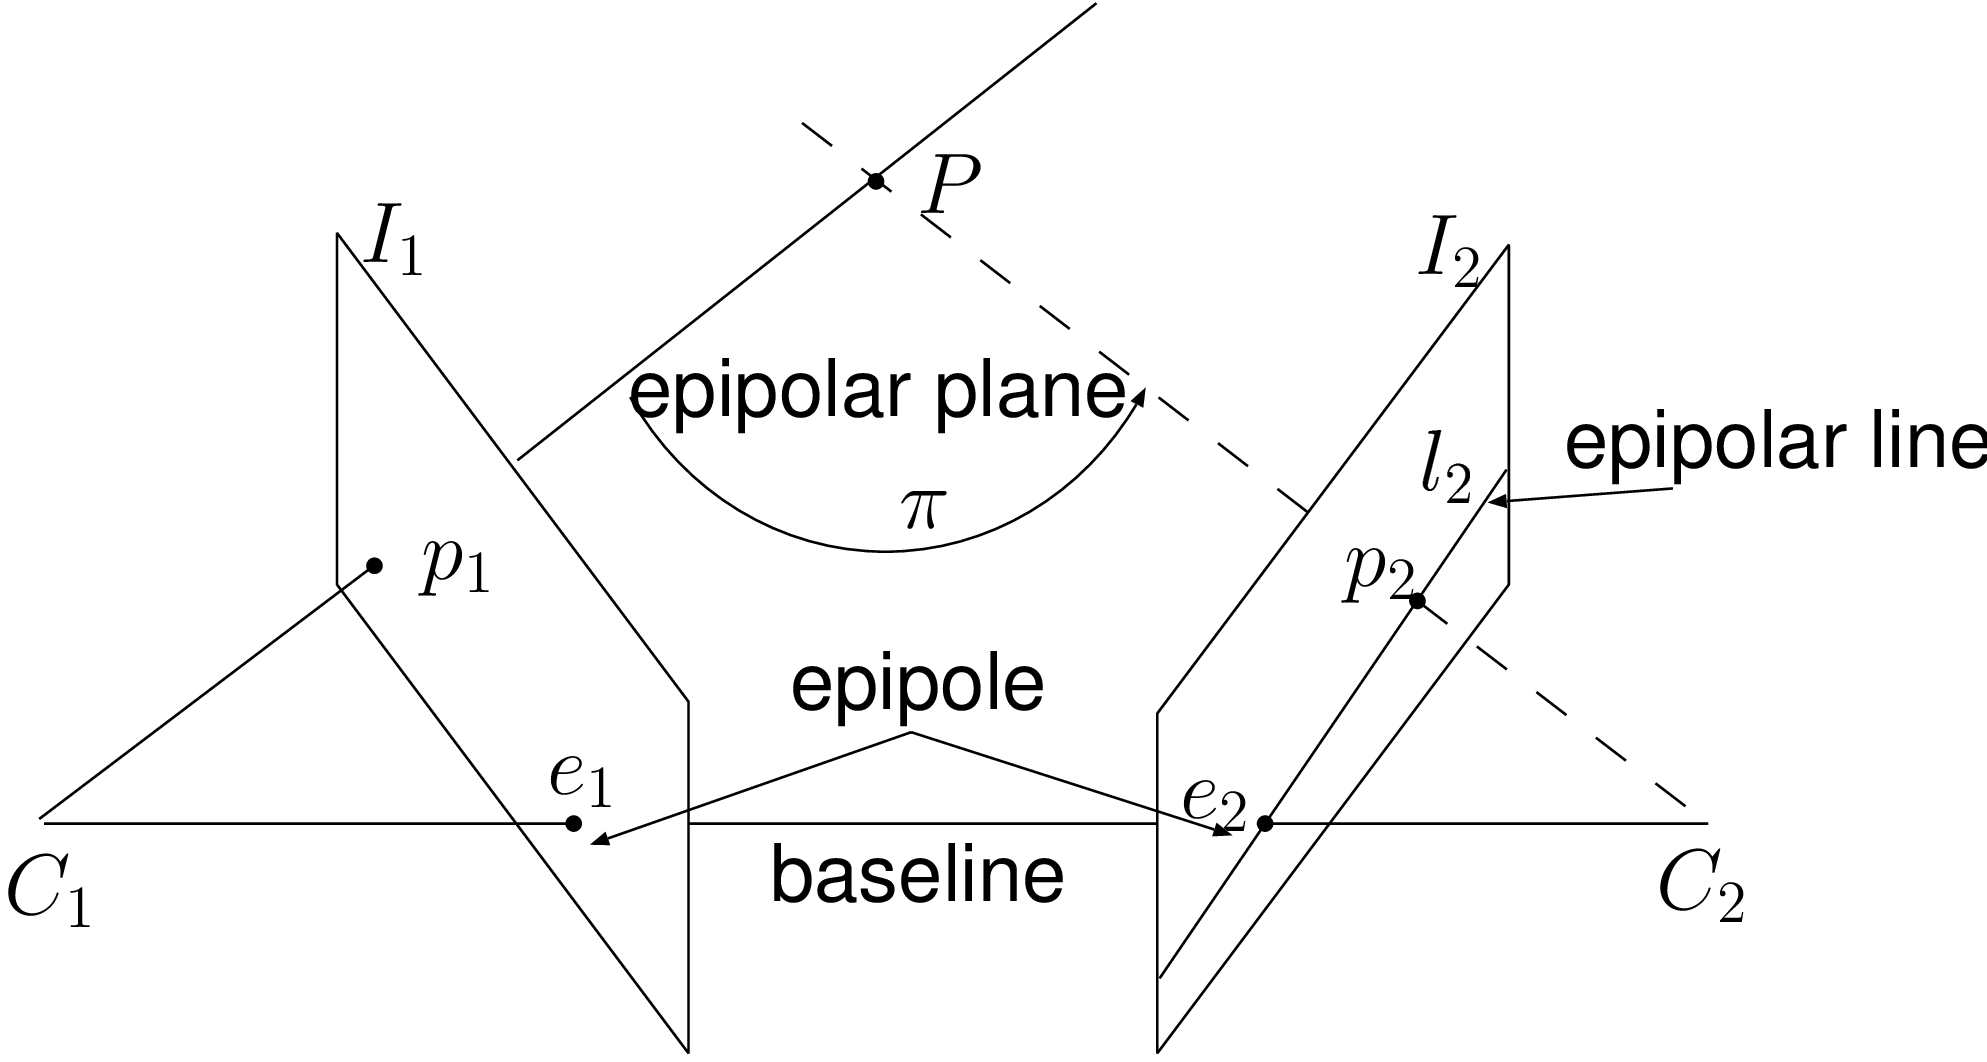
\includegraphics[width=.8\textwidth]{images/epipolar-geometry}}
\caption{Epipolar geometry}
\label{fig:epipolargeom}
	\end{center}
\end{figure}
Main goal of epipolar geometry is the computation of pixels correspondences among the input images. 
Neighbouring pixels information, cameras positions and their calibration data are fundamental to achieve that.
Figure \ref{fig:epipolargeom} demonstrate a pixel in one image $\mathbf{p}_1$ projected to its correspondent epipolar line segment in the other image, which is lower bounded by the projection of the first camera center into the second camera plane, i.e. the epipole $\mathbf{e}_2$. 
Projecting the epipolar line in the second image back to the first, another line would be obtained, bounded by the correspondent epipole $\mathbf{e}_1$. 
The extensions to infinity of these two segment are identified as the epipolar lines, which are defined by the intersection of the two image planes with the epipolar plane.
A fundamental property is that the epipolar plane passes through both camera centers $\mathbf{C}_1$ and $\mathbf{C}_2$, as well as point $\mathbf{P}$. 
Therefore, they lie in the same plane. \\

\subsection{Rectification}
\label{subsection:rectification}
\begin{figure}[t]
	\begin{center}
		{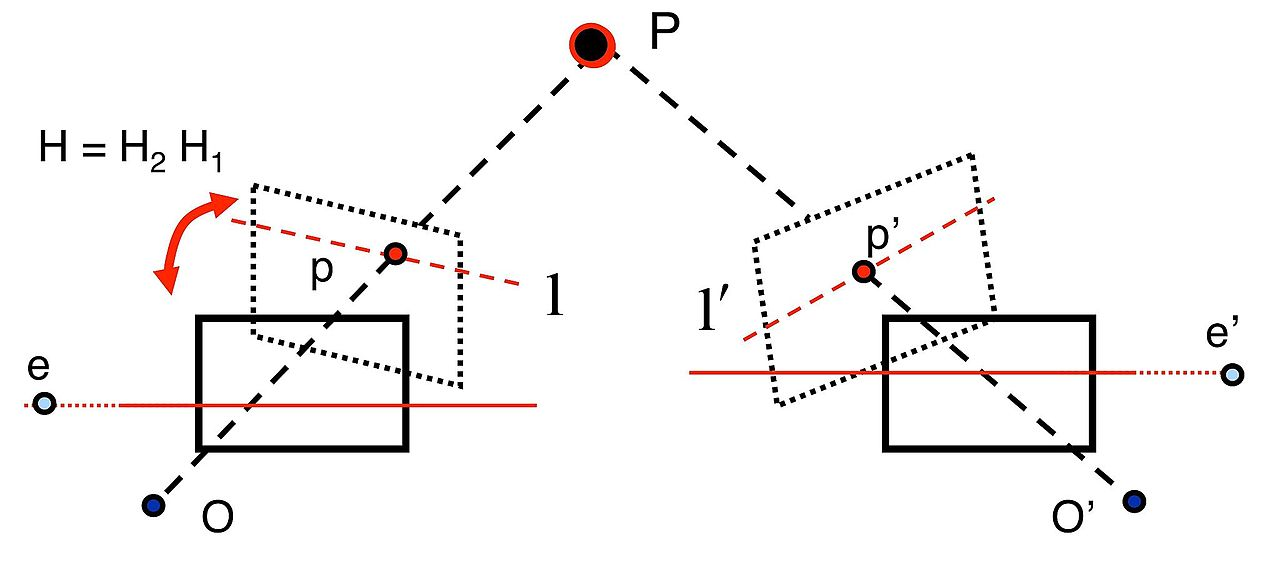
\includegraphics[width=.8\textwidth]{images/rectification}}
\caption{Image rectification -- Source: L. Lebeznik}
\label{fig:rectification}
	\end{center}
\end{figure}

Epipolar geometry for a pair of cameras is relative to pose and calibration of the camera and can be computed using the fundamental matrix, which can be obtained applying the eight point algorithm \citep{hartley2004multiple}.
Computing this geometry allows, then, to find the correspondent pixels between the two images using the constraint of the epipolar lines.
This is possible, because, as explained in \ref{subsection:stereogeom}, considered a pixel in one image, the correspondent one lies on the relative epipolar line.\\
Beside that, pixels correlations can be more efficiently performed by rectifying the input images \citep{hartley2004multiple}.
In Figure \ref{fig:rectification} is clearly visible the outcome of this process and its advantages.
As shown, corresponding horizontal scanlines are epipolar lines. 
The essential importance of this standard rectified geometry is clearly explained by the following equation,
\begin{equation} \label{eqn:disparity-depth}
	d = f \frac{B}{Z}
\end{equation}

that leads to a linear relationship between 3D depth $Z$ and disparity $d$, where $f$ is the focal length (in pixel) and $B$ the baseline.
Moreover, the relationship between the corresponding pixels in the left and right images can be defined as follows:
\begin{equation} \label{eqn:corresponding-pixel}
	x' = x + d(x, y), \; y' = y
\end{equation}

Thus, the main step for recovering a depth image of a scene is the estimation of the disparity map $d(x,y)$.\\
As introduced at the beginning, the best disparity map is estimated after the rectification process. 
This is performed by comparing the similarity of corresponding pixels, as defined in equation \ref{eqn:corresponding-pixel}, and storing them in a disparity space image $C(x,y,d)$, which is then processed with multiple algorithms. 

\subsection{Stereo methods and dense correspondence}
\label{stereomethods}
In this section a brief delineation of the general pipeline implemented in most of the stereo matching method is presented. 
Moreover, as a theoretical completion of what introduced above, some generic algorithm are further explained.\\
Stereo algorithm follows in general a subspace of the following methods: matching cost computation, cost aggregation, disparity computation and optimization and disparity refinement \citep{Scharstein2001}.\\
A preliminary distinction, based on those phases, separates stereo methods between local or window-base global methods.\\
In local methods, the disparity computation in a certain region depends on the pixel intensities within a limited window.\\
On the contrary, global algorithms, are based on an energy function.
In this one smoothness assumptions are defined and then a global optimization problem is solved. 
These algorithm are mainly distinguished considering the minimization strategy, such that, simulated annealing, graph cuts or belief propagation.\\
Between these two classes there are iterative and hierarchical algorithms. 
The latter aim to constraint gradually the disparity estimation from the coarser to the finer levels \citep{Hirschmuller2008}.\\
Considering the first general step of stereo matching algorithms, the matching cost, there are multiple measures to define it.
Among the most prevalent pixel-based algorithm can be included square intensity differences, absolute intensity differences, mean-squared error and mean absolute difference.\\
Other common matching cost comprehend normalized cross-correlation, which is similar to sum-of-squared-difference (SSD), and binary methods. 
However, the latter tend to not be used any longer. \\
On the other hand, lately, more robust algorithms are used for their insensitivity to non-stationary exposure and illumination changes. 
Entropy measures and non-parametric functions such as, rank and census transform \citep{Zabih1994}, sampling insensitive difference\citep{Birchfield1999} and hierarchical mutual information \citep{Hirschmuller2008}, are some examples.
In particular, they allow to obtain accurate performance when considerable exposure or appearance variations are present. \\
Drawing up some conclusion regarding the local methods, the core steps are the matching cost calculation and the aggregation phase. 
Disparity estimation, then, becomes trivial. Each pixel takes the disparity levels whose cost value is the minimum. 
This approach is said to be a local \textit{winner-take-all} optimization. 
A drawback of this approach is that the matches are imposed for the reference image. 
While points is the support image might have multiple correct matches. 
For this reason, cross-checking and post-processing become more relevant here.\\
Summarizing the general pipeline of global stereo matching methods, they often get rid of the aggregation step. 
They usually perform sort of optimization steps after disparity estimation, exploiting the smoothness constraints as aggregation part. \\
Goal of this approach is to find the solution to a global energy function, i.e. the disparity $d$ that minimizes the energy,
\begin{equation}\label{eqn:energyfct}
	E(d) = E_d(d) + \lambda E_s(d)
\end{equation}
where $E_d(d)$ is the data term and $E_s(d)$ the smoothness term.
Adopting the aforementioned disparity space image (DSI) matching cost, the data energy is calculated as:
\begin{equation}\label{dataterm}
	E_d(d) = \sum_{(x,y)} C(x, y, d(x, y))
\end{equation}
where $C$ is the DSI.
Then, the smoothness term is usually defined as:
\begin{equation}\label{smoothterm}
	E_s(d) = \sum_{(x,y)} \rho (d(x,y) - d(x + 1, y)) + \rho (d(x,y) - d(x, y + 1))
\end{equation}
where $\rho$ is some monotonically increasing function of disparity difference. \\
After the energy function has been clearly identified, different categories of algorithms can be exploited to recover a (local) minimum.
Graph cut, belief propagation and Markov random field (MRF) based methods have been proved to give the most accurate results. 


\section{Structure of the Thesis}
\label{section:structure} 

You should use transition in your text, meaning that you should help
the reader follow the thesis outline. Here, you tell what will be in
each chapter of your thesis. Often the thesis does not have as many
chapters as is in this template. For example, environment and
implementation can be combined as well as chapters of evaluation and
discussion.  The rest of this thesis is organized as
follows. Chapter~\ref{chapter:background} gives the background, etc.

